\section{Experiments}
\begin{figure}[htp!]
    \centering
    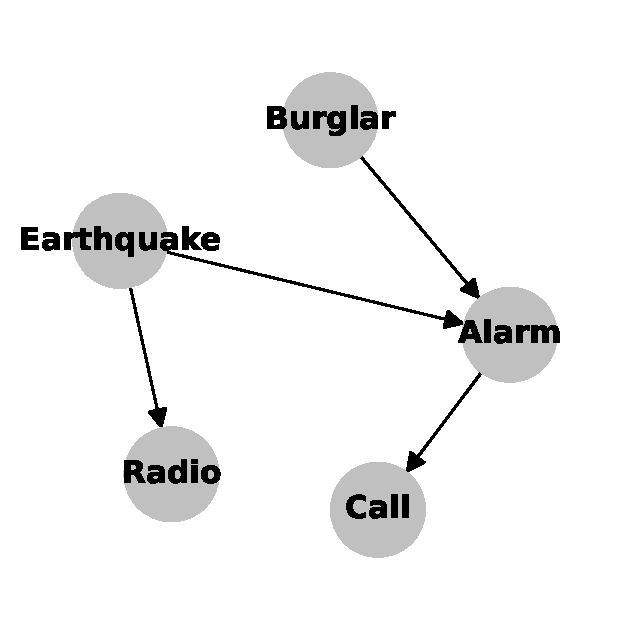
\includegraphics[width=0.5\linewidth]{plots/alarm.pdf}
    \caption{An example of a Bayesian Network to learn}
    \label{fig:alarm_fig}
\end{figure}
\begin{figure}[htp!]
     \centering
     \begin{subfigure}{0.7\textwidth}
         \centering
    
\includegraphics[width=\textwidth]{plots/legends.pdf}
     \end{subfigure}
     \begin{subfigure}{0.32\textwidth}
         \centering
         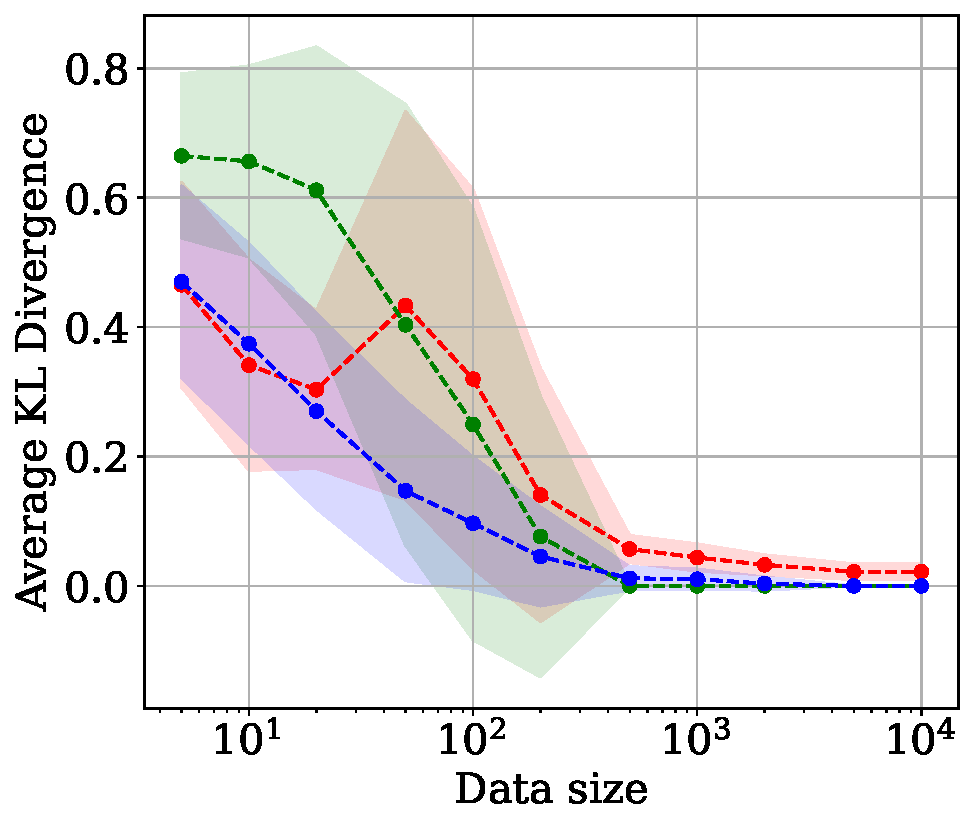
\includegraphics[width=\textwidth]{plots/kl_divergence.pdf}
         \caption{KL divergence between the probability distributions learned by the model and that observed in the data.}
         \label{fig:kl_div_dist}
     \end{subfigure}
     \hfill
     \begin{subfigure}{0.32\textwidth}
         \centering
         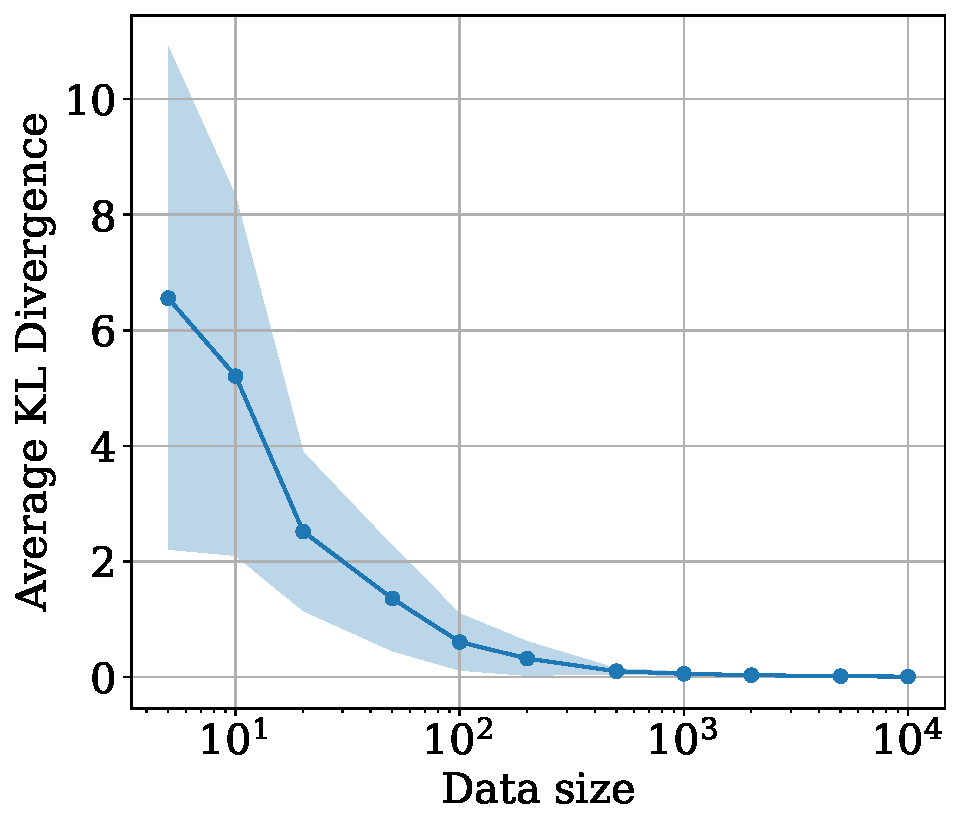
\includegraphics[width=\textwidth]{plots/joint_dist_div.pdf}
         \caption{KL divergence between the joint distributions observed from the samples from the model and that observed in the data.}
         \label{fig:kl_div_joint}
     \end{subfigure}
     \hfill
     \begin{subfigure}{0.32\textwidth}
         \centering
         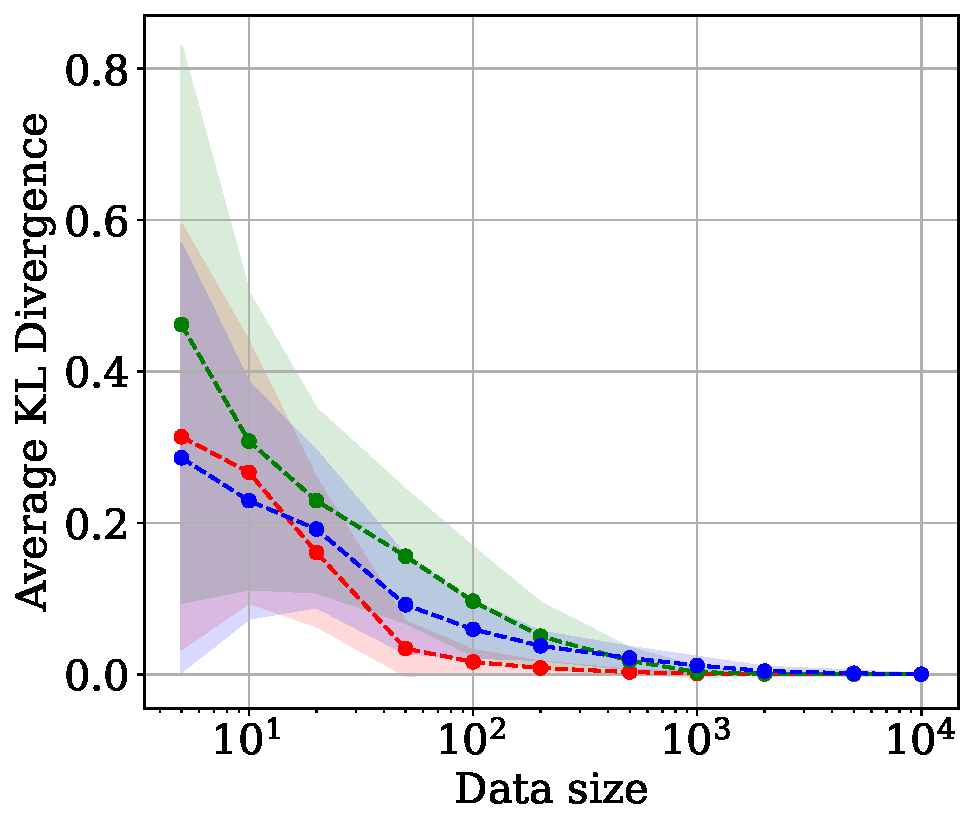
\includegraphics[width=\textwidth]{plots/marginals_kl_divergence.pdf}
         \caption{KL divergence between the marginal distributions observed from the samples from the model and that observed in the data.}
         \label{fig:kl_div_marginals}
     \end{subfigure}
        \caption{Comparison of Exact algorithm and Chow-Liu approximation algorithm for learning Bayesian networks from discrete data.}
        \label{fig:str_learning_comp}
\end{figure}

\begin{figure}[htp!]
\begin{subfigure}{0.7\textwidth}
         \centering
    
\includegraphics[width=\textwidth]{plots/legends.pdf}
     \end{subfigure}
    \centering
    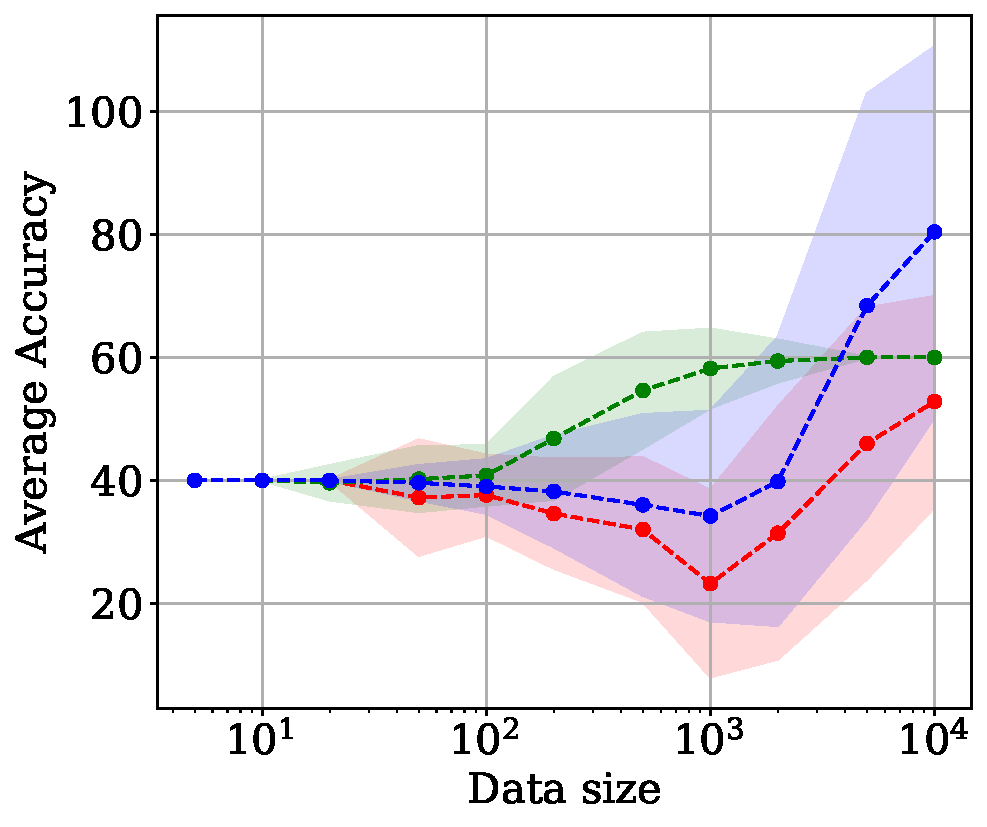
\includegraphics[width=0.5\linewidth]{plots/accuracy.pdf}
    \caption{Comparison of structural accuracy using Exact learning and Chow-Liu approximation learning}
    \label{fig:str_acc}
\end{figure}

% \begin{figure*}
%     \centering
%     \begin{minipage}{\textwidth}
%     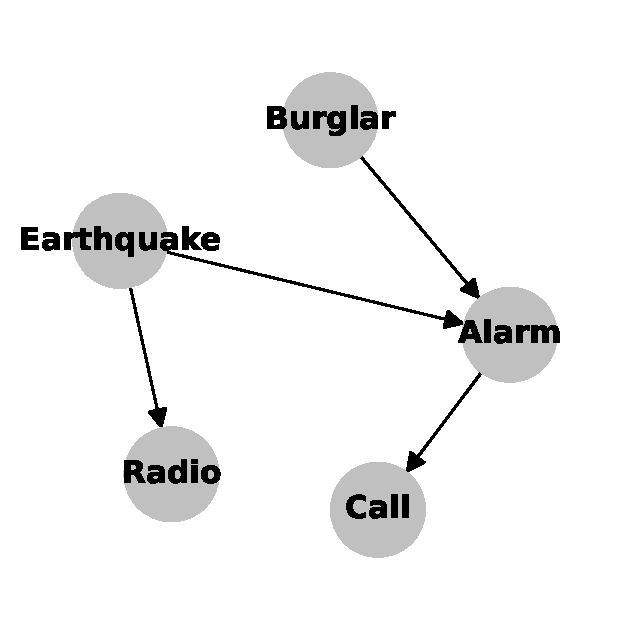
\includegraphics[width = \linewidth]{plots/alarm.pdf}
%     \end{minipage}
%     \begin{minipage}{0.32\textwidth}
%     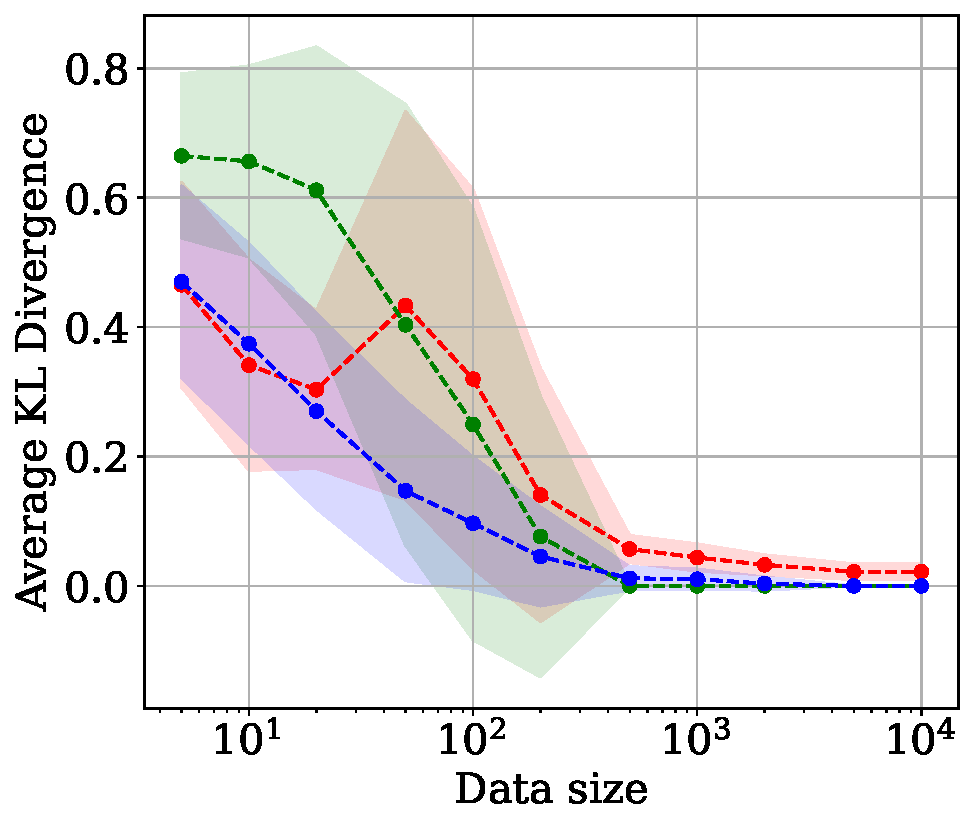
\includegraphics[width = \linewidth]{plots/kl_divergence.pdf}
%     % \caption{a}
%     \end{minipage}
%     \begin{minipage}{0.32\textwidth}
%     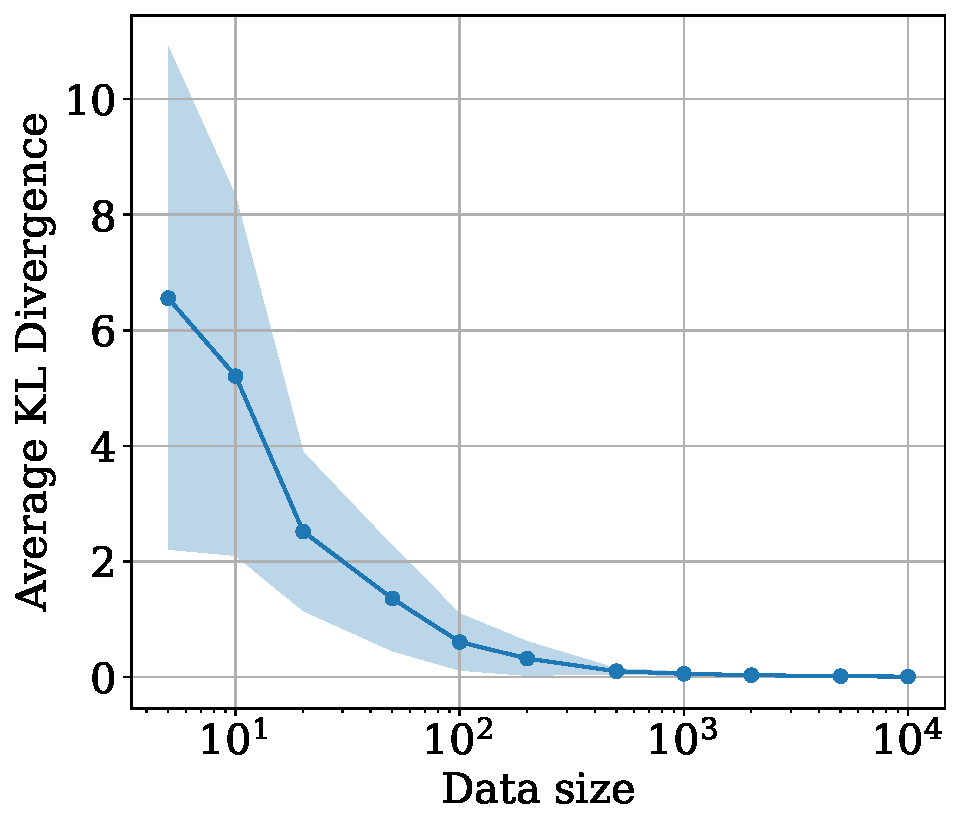
\includegraphics[width = \linewidth]{plots/joint_dist_div.pdf}
%     % \caption{b}
%     \end{minipage}
%     \begin{minipage}{0.32\textwidth}
%     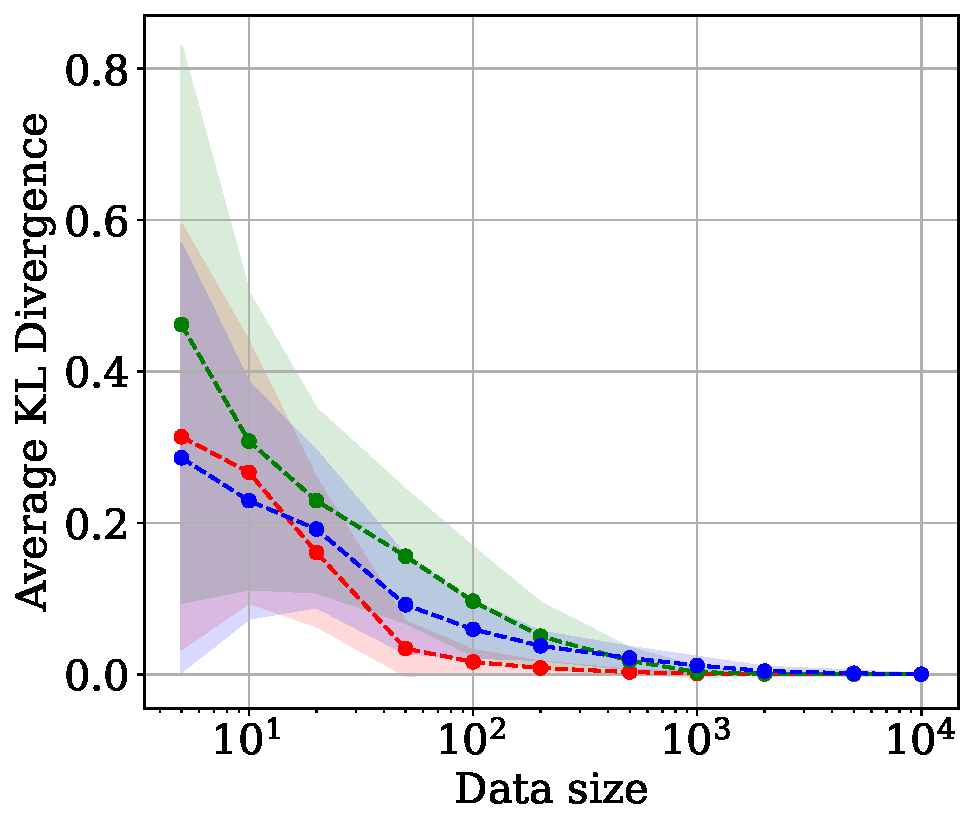
\includegraphics[width = \linewidth]{plots/marginals_kl_divergence.pdf}
%     % \caption{c}
%     \end{minipage}
%     \caption{To fill up later}
%     \label{fig:kl_div}
% \end{figure*}

% \begin{figure*}
% \centering
%     \begin{minipage}{0.45\textwidth}
%     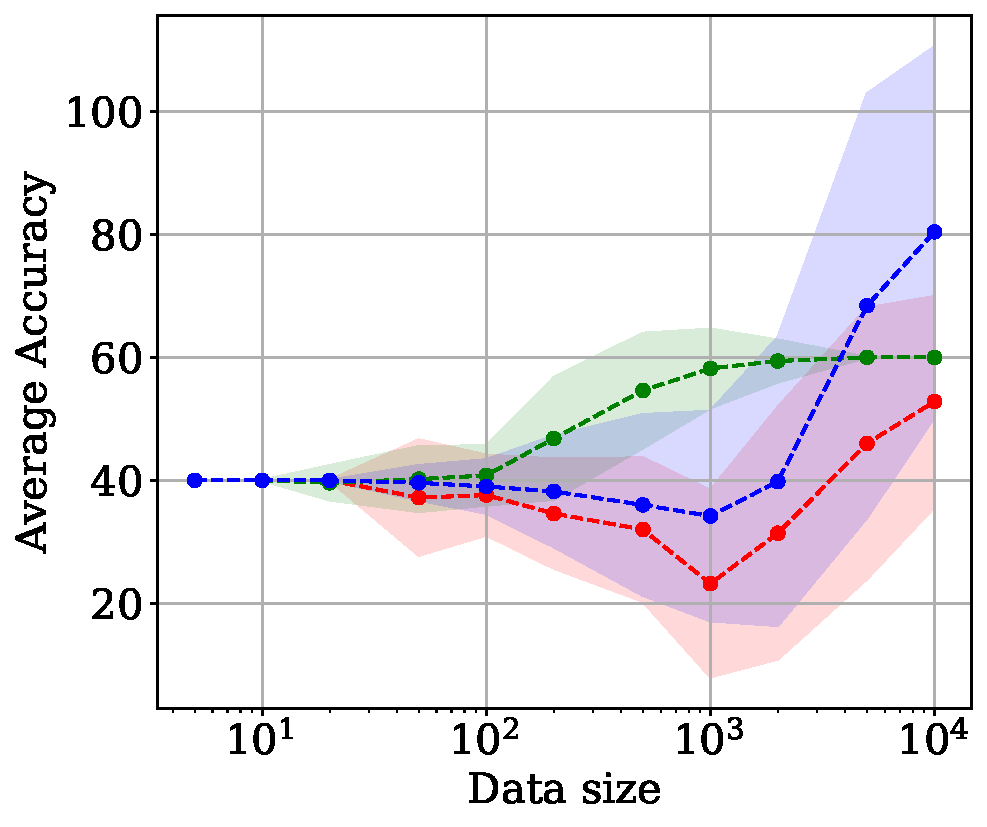
\includegraphics[width = \linewidth]{plots/accuracy.pdf}
%     % \caption{Test 1}
%     \end{minipage}
% \end{figure*}